\subsection{Calibration stability across the run}

\begin{figure}[ht]
\begin{center}
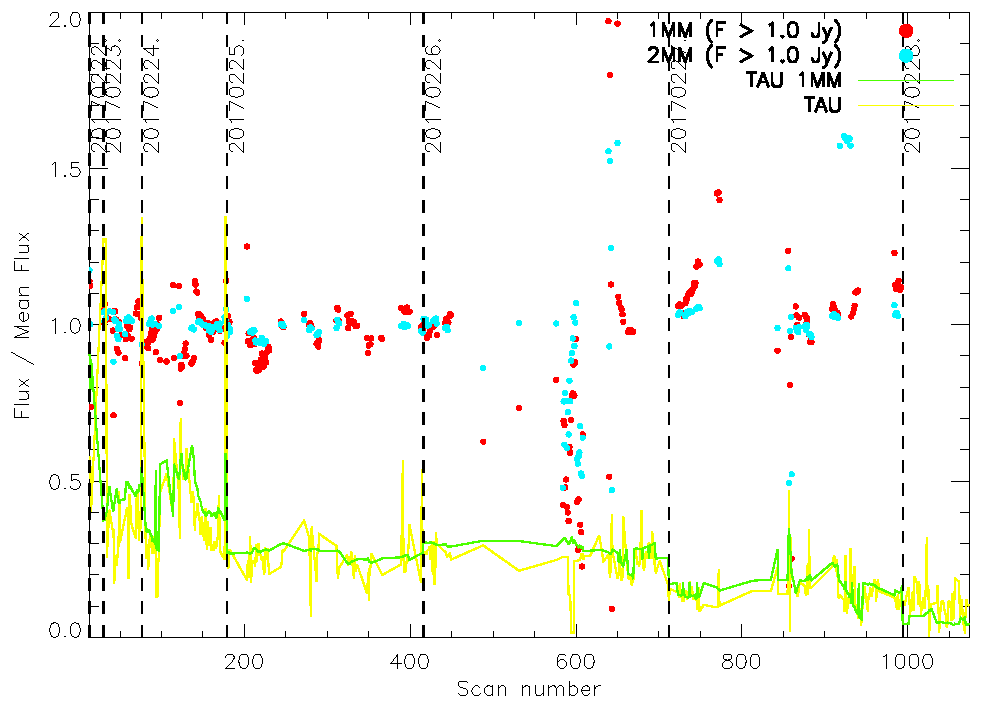
\includegraphics[clip, angle=0, scale = 0.7]{Figures/FluxIndScans/flux_ratio_run22.pdf}
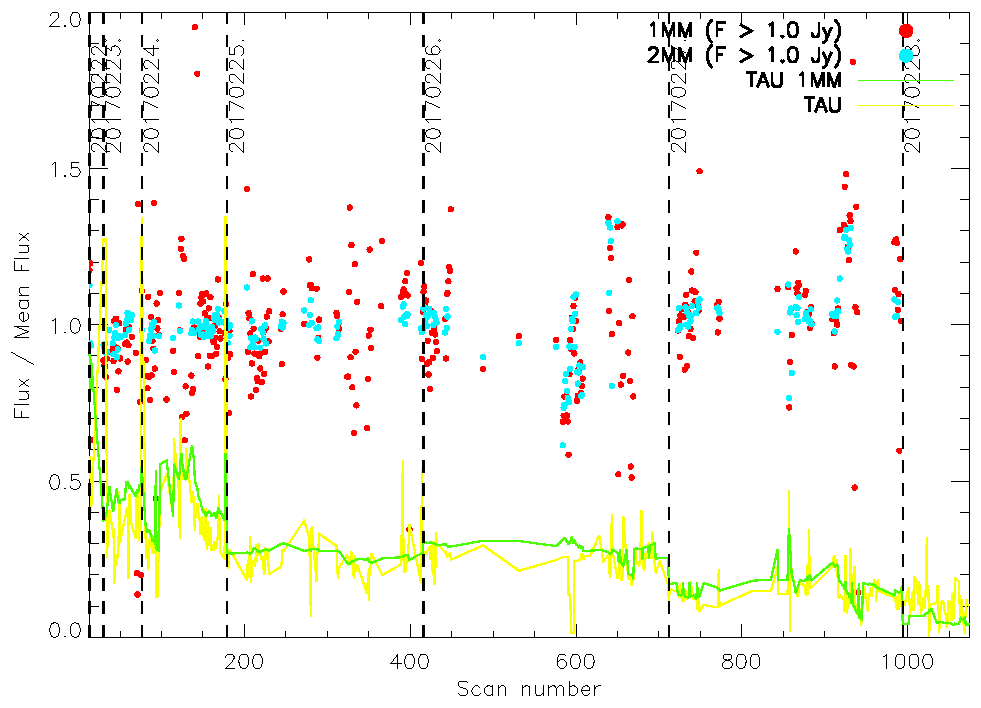
\includegraphics[clip, angle=0, scale = 0.7]{Figures/FluxIndScans/flux_ap_ratio_run22.pdf}
\caption{Ratio between the measured flux per scan and the averaged flux for all sources observed in N2R9. We considered both fixed FWHM (top) and aperture photometry fluxes for the 1 (red) and 2 (cyan) mm channels. }
\label{fig:fluxvsscan}
\end{center}
\end{figure}

\begin{figure}[ht]
\begin{center}
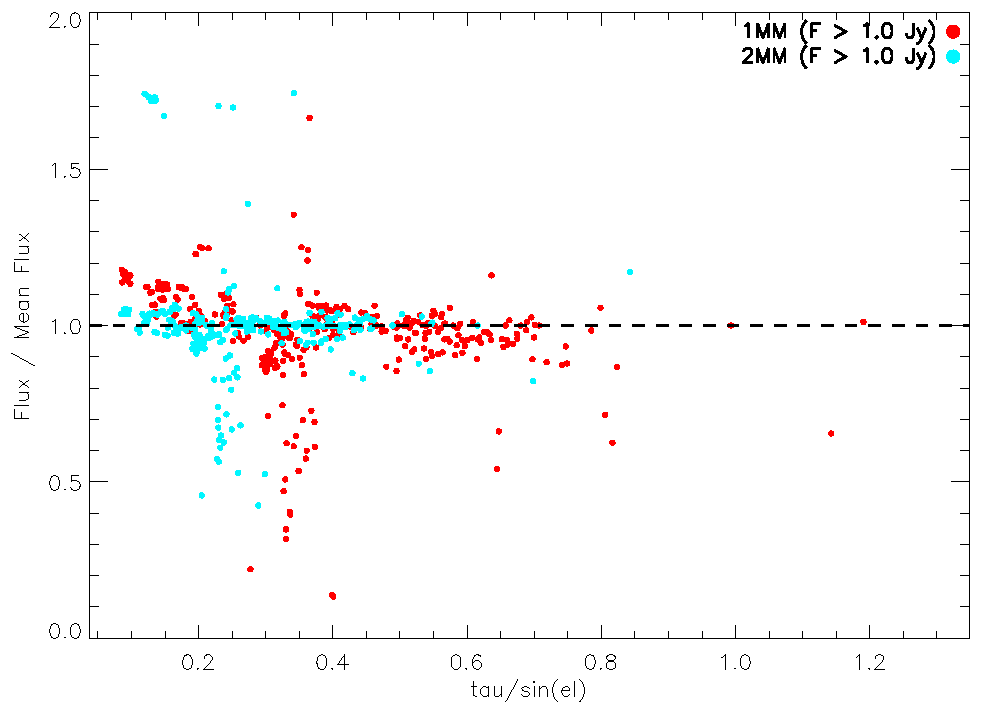
\includegraphics[clip, angle=0, scale = 0.7]{Figures/FluxIndScans/flux_ratio_rz_run22.pdf}
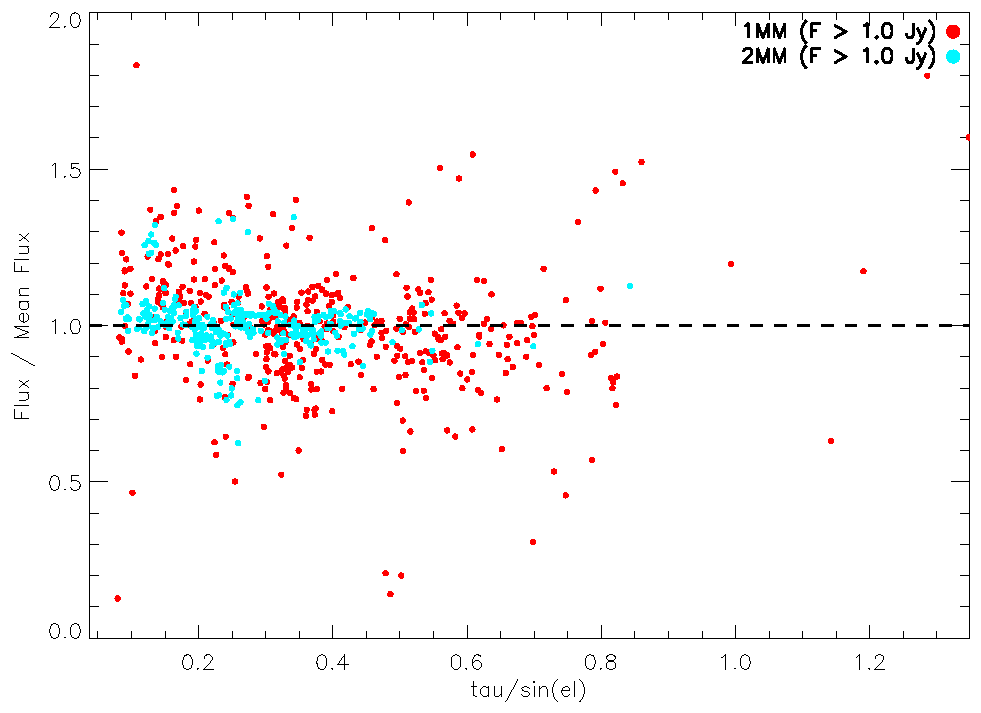
\includegraphics[clip, angle=0, scale = 0.7]{Figures/FluxIndScans/flux_ap_ratio_rz_run22.pdf}
\caption{Ratio between the measured flux per scan and the averaged flux as a function atmospheric backgroud for all sources observed in N2R9. We considered both fixed FWHM (top) and aperture photometry fluxes for the 1 (red) and 2 (cyan) mm channels. }
\label{fig:fluxvsbackground}
\end{center}
\end{figure}
